%\documentstyle[epsf,twocolumn]{jarticle}       %LaTeX2.09�d�l
\documentclass[twocolumn]{jarticle}
%%%%%%%%%%%%%%%%%%%%%%%%%%%%%%%%%%%%%%%%%%%%%%%%%%%%%%%%%%%%%%
%%
%%
%%
%%%%%%%%%%%%%%%%%%%%%%%%%%%%%%%%%%%%%%%%%%%%%%%%%%%%%%%%%%%%%%%%
\setlength{\topmargin}{-45pt}
%\setlength{\oddsidemargin}{0cm}
\setlength{\oddsidemargin}{-7.5mm}
%\setlength{\evensidemargin}{0cm}
\setlength{\textheight}{24.1cm}
%setlength{\textheight}{25cm}
\setlength{\textwidth}{17.4cm}
%\setlength{\textwidth}{172mm}
\setlength{\columnsep}{11mm}
%\setlength{\intextsep}{0pt}
%\setlength{\floatsep}{0pt}
%\setlength{\textfloatsep}{0pt}
%\makeatletter
%\renewcommand{\theequation}{%
%\thesection.\arabic{equation}} %\@addtoreset{equation}{section}
%\makeatother

%\renewcommand{\arraystretch}{0.95}

%%%%%%%%%%%%%%%%%%%%%%%%%%%%%%%%%%%%%%%%%%%%%%%%%%%%%%%%
\usepackage{graphicx}
\usepackage[dvipdfmx]{color}
\usepackage{diagbox}
\usepackage{float}
\usepackage[margin=20truemm]{geometry}
\usepackage{multirow}
\usepackage{subcaption}
\usepackage{listings}
\usepackage{xcolor}
%%%%%%%%%%%%%%%%%%%%%%%%%%%%%%%%%%%%%%%%%%%%%%%%%%%%%%%%

\begin{document}
\twocolumn[
  \noindent

  \hspace{1em}

  後期研究会発表資料 令和 6 年 12 月 2 日 (月)
  \hfill
  \ \ M2 高山 裕成

  \vspace{2mm}

  \hrule

  \begin{center}
    {\Large \bf BERT を用いた原文と要約文の分散表現の最適な統合手法の検討}
  \end{center}


  \hrule
  \vspace{3mm}
]

\lstset{
  basicstyle=\ttfamily\scriptsize, % フォント設定
  backgroundcolor=\color{white},  % 背景色
  frame=single,                     % 枠線
  breaklines=true,                  % 長い行を折り返し
  breakatwhitespace=true,           % 空白で折り返し
  breakautoindent=false,             % 折り返し時にインデントを自動調整
}

% 脚注番号を *1, *2 のように表示する設定
\renewcommand{\thefootnote}{*\arabic{footnote}}

\section{はじめに}
近年, 深層学習をはじめとする機械学習手法は目覚ましい発展を遂げており, 自然言語処理や画像処理などの分野で高い精度を達成している.

より高精度なモデルを作るための深層学習の要素技術の 1 つにプーリングと呼ばれる手法がある. プーリングとは, 入力されたデータから得た特徴量の次元を縮小し, 計算量を削減するとともに, 抽出された特徴量のロバスト性を高めるための手法である. しかし, 自然言語処理分野におけるプーリング手法は画像処理分野と比べて数少なく, その効果に関する理解は不十分であるという背景がある. このような背景を踏まえ, 大和\cite{yamato}は大規模言語モデル (Large Language Models, LLM) の 1 つである BERT において一般的に用いられる [CLS] トークンの埋め込み表現を用いたプーリング手法と, 平均プーリング手法を組み合わせた CLS-Average Pooling (CAP 層) を提案し, テキスト分類タスクにおける各プーリング手法のみを用いた場合と比較して, その有効性を示した.

本研究では, 大和による手法を基に, LLM を用いて原文から生成した要約文の分散表現を組み込んだ新たなプーリング手法を検討し, テキスト分類タスクにおける性能向上を目的とした.


\section{要素技術}
\subsection{BERT}
Bidirectional Encoder Representations from Transformers (BERT) \cite{devlin-etal-2019-bert} は, 2018 年に
Google が発表した複数層の双方向 Transformer エンコーダに基づく汎用言語モデルである.
BERT は, 入力された単語列全体に対応する分散表現と, 入力された単語列の各単語に対応する分散表現を出力する. 事前学習済みモデルを他のタスクに転移学習することが容易で
, さまざまなタスクに対応することができる.

本研究では, 東北大学の乾研究室から公開されている日本語版 Wikipedia と CC-100 データセットの日本語部分で事前学習されたモデル\footnote{ https://huggingface.co/cl-tohoku/bert-base-japanese-v3}を用いた.

\subsection{PLaMo}
PLaMo\footnote{ Preferred Elements, https://plamo.preferredai.jp/, 2024.} は Preferred Elements 社が開発している大規模言語モデルである. 多言語に広く対応している Generative Pre-trained Transformer (GPT)\cite{radford2018improving} とは異なり, 日本語に特化した独自のテキストデータを中心に事前学習されており, 他社モデルをベースとしていないため, 社外ライセンスの縛りや開発上における不明瞭点が取り除かれている国産の基盤モデルである.

\section{先行研究}
図\ref{fig:1_cap} に大和\cite{yamato}による CAP 層の概略を示す. 図\ref{fig:1_cap} のように,
BERT におけるテキスト分類で一般的に用いられる [CLS] トークンの埋め込み表現 $E_{\rm{[CLS]}}$ および, [CLS] トークン以外の入力トークンすべてに対する平均プーリングによって得られた埋め込み表現 $E_{\rm{Avg}}$ に対して, 学習可能な和が 1 となるパラメータ $p, q (\geq0)$ を用いて $E_{\rm{[CLS]}}$ および, $E_{\rm{Avg}}$ の重み付き和
\begin{equation}
  pE_{\rm{[CLS]}}+qE_{\rm{Avg}}
\end{equation}
を CAP 層の出力とし, 入力データの分散表現とする. また, 重みパラメータ $p, q$ の更新式は更新後の値を $p', q'$ とすると以下の式で表される.
\begin{equation}
  p' = \frac{p^{2}}{p^{2}+q^{2}}
\end{equation}
\begin{equation}
  q' = \frac{q^{2}}{p^{2}+q^{2}}
\end{equation}


\begin{figure}[b]
  \begin{center}
    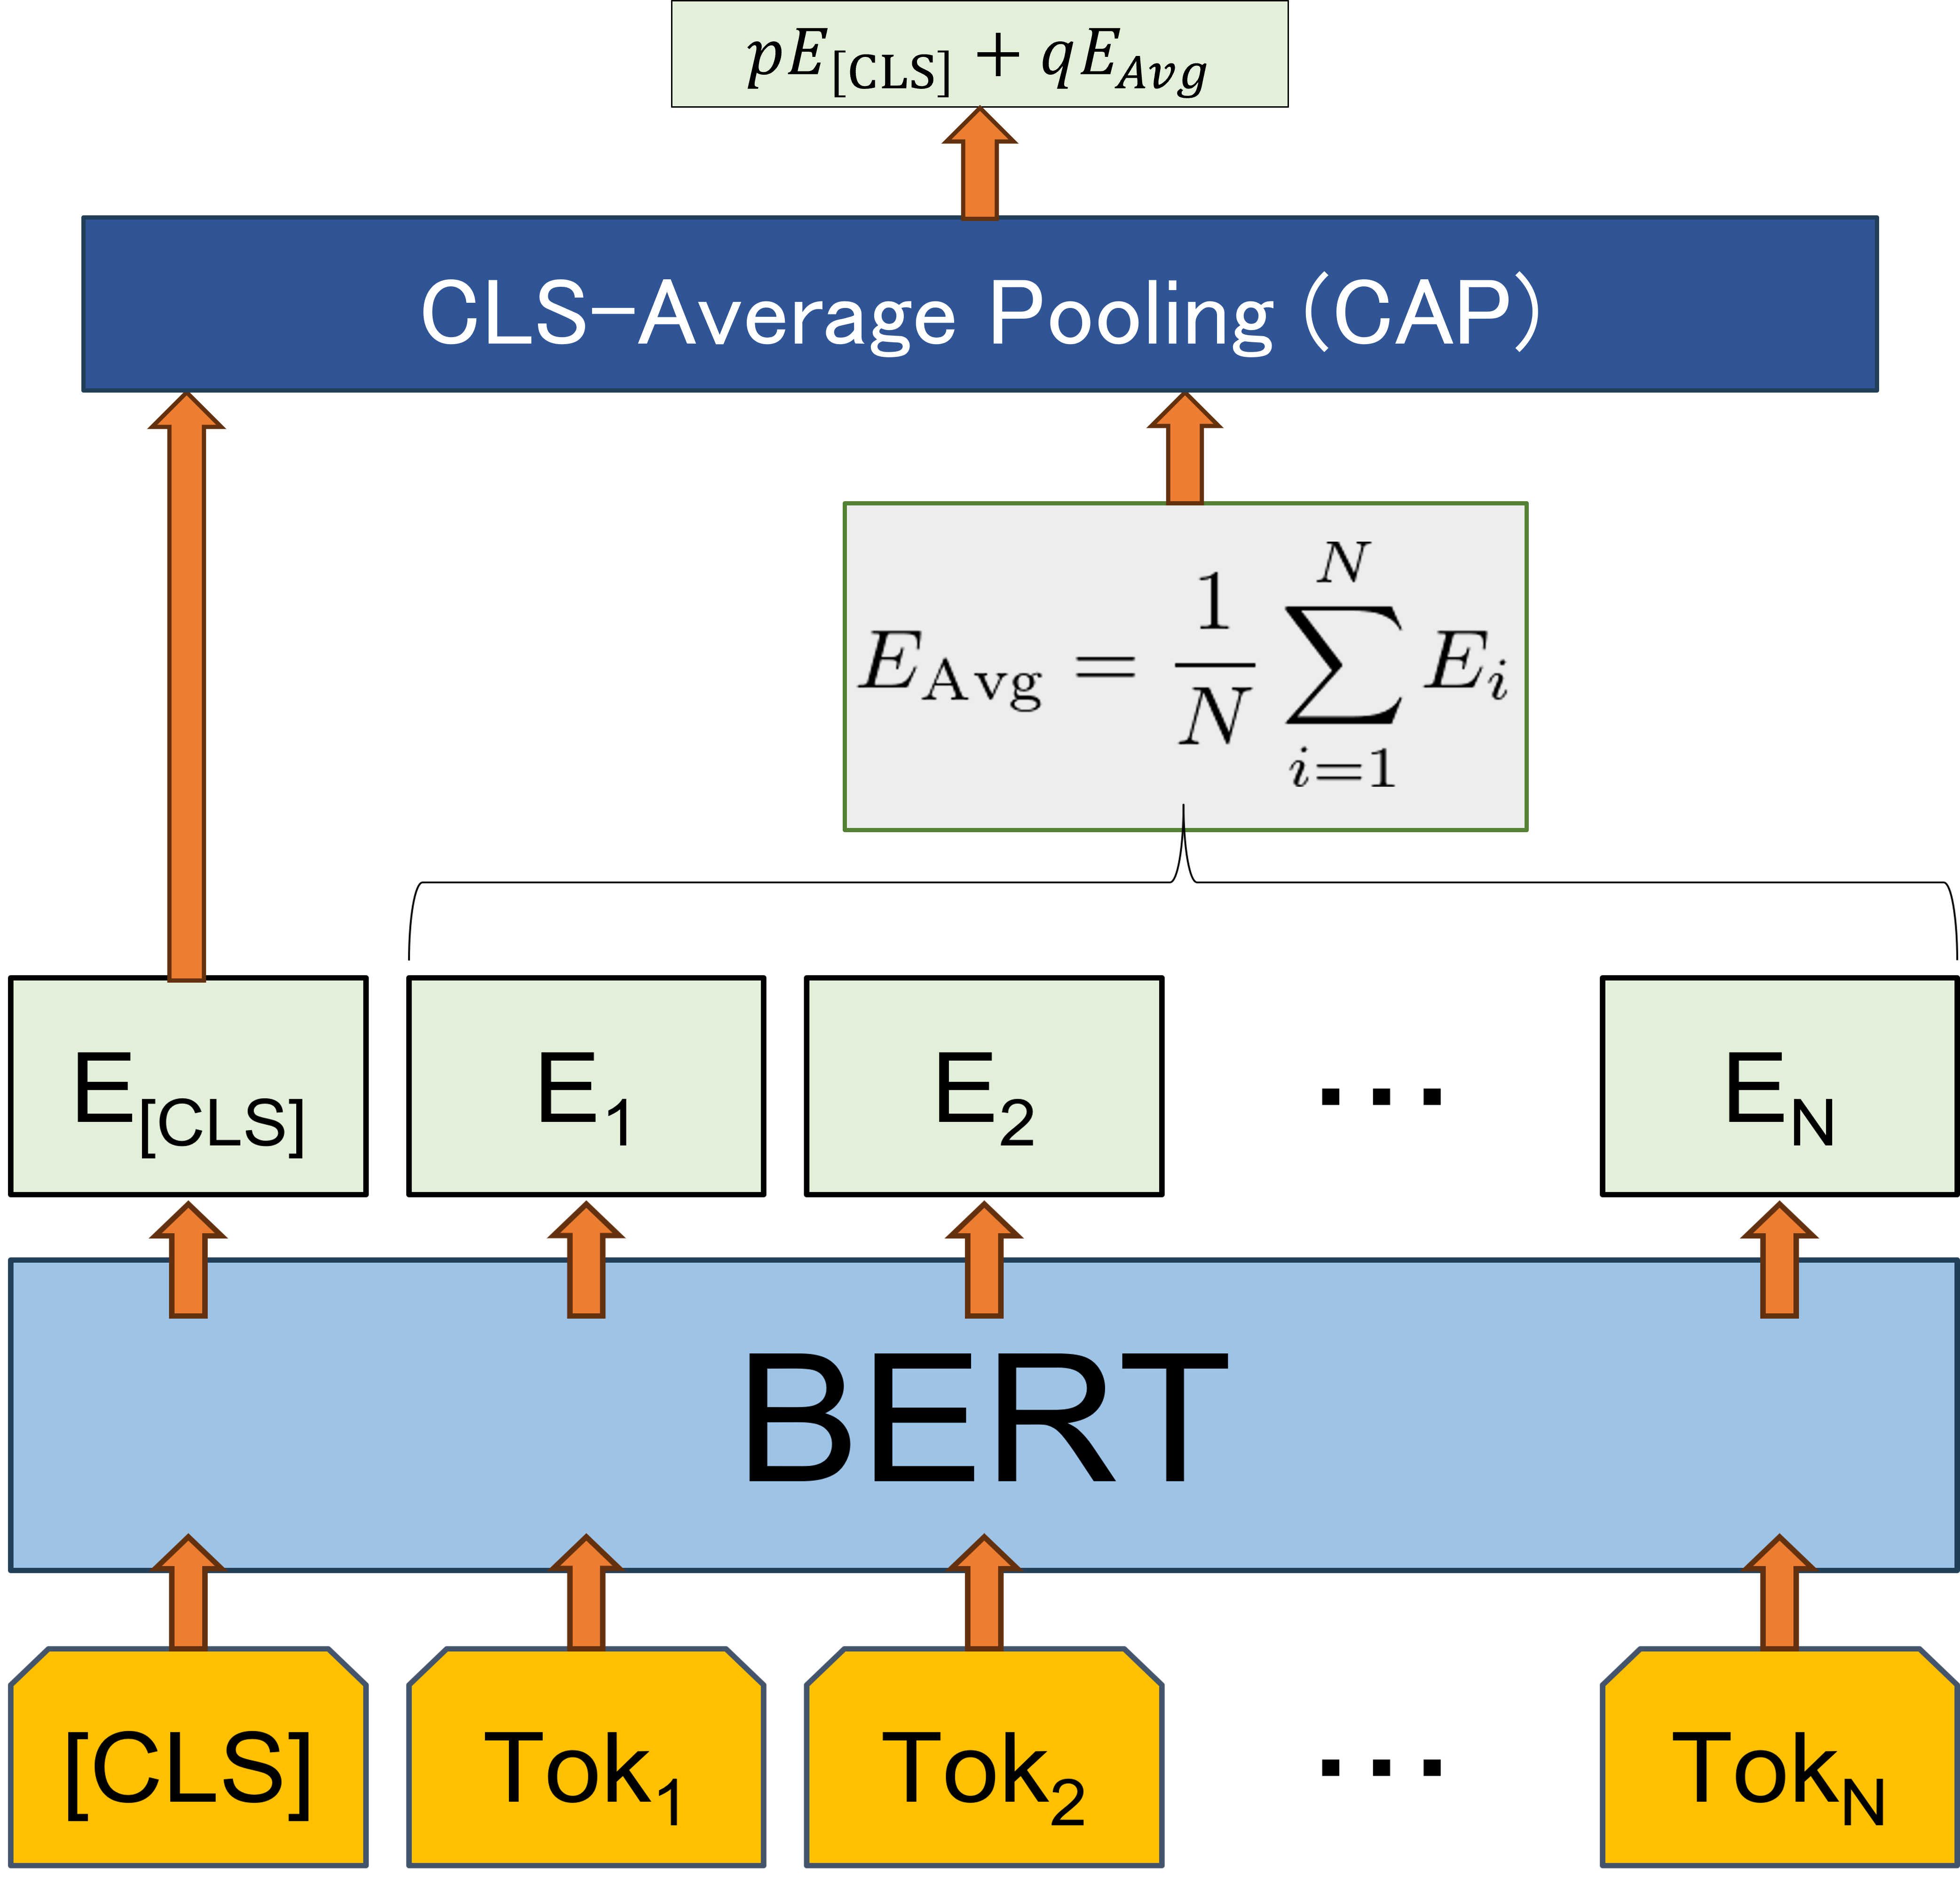
\includegraphics[width=0.65\linewidth]{cap.png}
    \caption{CLS-Average Pooling (CAP 層) の概要} %タイトルをつける
    \label{fig:1_cap} %ラベルをつけ図の参照を可能にする
  \end{center}
\end{figure}

\newpage

\section{データセット}
本研究では, 先行研究に倣い livedoor ニュースコーパス\footnote{ http://www.rondhuit.com/download.html} を用いた. これは, 株式会社ロンウィットが公開しているデータセットであり, オンラインニュースサイト「livedoor ニュース」の記事を収集し, 可能な限り HTML タグを取り除いて作成されたコーパスである. 9 つのカテゴリ, 計 7367 記事から構成され, 各記事データ $\rm{D}$ はカテゴリ名 $\rm{D_{\rm{label}}}$, 記事タイトル $\rm{D_{\rm{title}}}$, 記事本文 $\rm{D_{\rm{body}}}$ などのメタデータから構成されている. 表\ref{tab:dataset} に実験で用いたデータセットの内訳を示す. 本研究では, 各カテゴリの記事を訓練データ, 検証データ, テストデータとして可能な限りラベル比が均等になるように 8:1:1 に分割した. 表\ref{tab:dataset} におけるラベルとカテゴリの対応は以下の通りである.

\begin{itemize}
  \item label 0 : 独女通信 (870 件)
  \item label 1 : IT ライフハック (870 件)
  \item label 2 : 家電チャンネル (864 件)
  \item label 3 : livedoor HOMME (511 件)
  \item label 4 : MOVIE ENTER (870 件)
  \item label 5 : Peachy (842 件)
  \item label 6 : エスマックス (870 件)
  \item label 7 : Sports Watch (900 件)
  \item label 8 : トピックニュース (770 件)
\end{itemize}

\begin{table*}[t]
  \centering
  \caption{データセットの内訳 (livedoor ニュースコーパス)}
  \scalebox{1.0}{
    \begin{tabular}{|c|c|c|c|c|c|c|c|c|c|c|}
    \hline
    & label 0 & label 1 & label 2 & label 3 & label 4 & label 5 & label 6 & label 7 & label 8 & Total \\
    \hline
    訓練 & 684 & 695 & 690 & 421 & 700 & 645 & 713 & 716 & 631 & 5895 \\
    \hline
    検証 & 88 & 80 & 88 & 42 & 93 & 100 & 77 & 105 & 63 & 736 \\
    \hline
    テスト & 98 & 95 & 86 & 48 & 77 & 97 & 80 & 79 & 76 & 736 \\
    \hline
    \end{tabular}%
  }
  \label{tab:dataset}%
\end{table*}%


\section{提案手法}
本研究では, PLaMo API を用いてデータセットに含まれるメタデータから各記事データ $\rm{D}$ の要約文を事前に生成し, 要約文から得た分散表現を CAP 層に組み込むプーリング手法について提案する. 図\ref{fig:2_teian} にモデルの概略を示す.

まず, 要約文の生成手法について説明する. 各記事データ $\rm{D}$ に対して, プロンプト $\rm{D_{\rm{prompt}}}$ を作成し, PLaMo からの回答 $\mathcal{L}(\rm{D_{\rm{prompt}}})$ を記事データ $\rm{D}$ の要約文 $\rm{D_{\rm{summary}}}$ とした. 図 \ref{fig:3_prompt} に要約文の生成プロンプトの概要を示す.

\begin{figure}[h]
  \begin{center}
    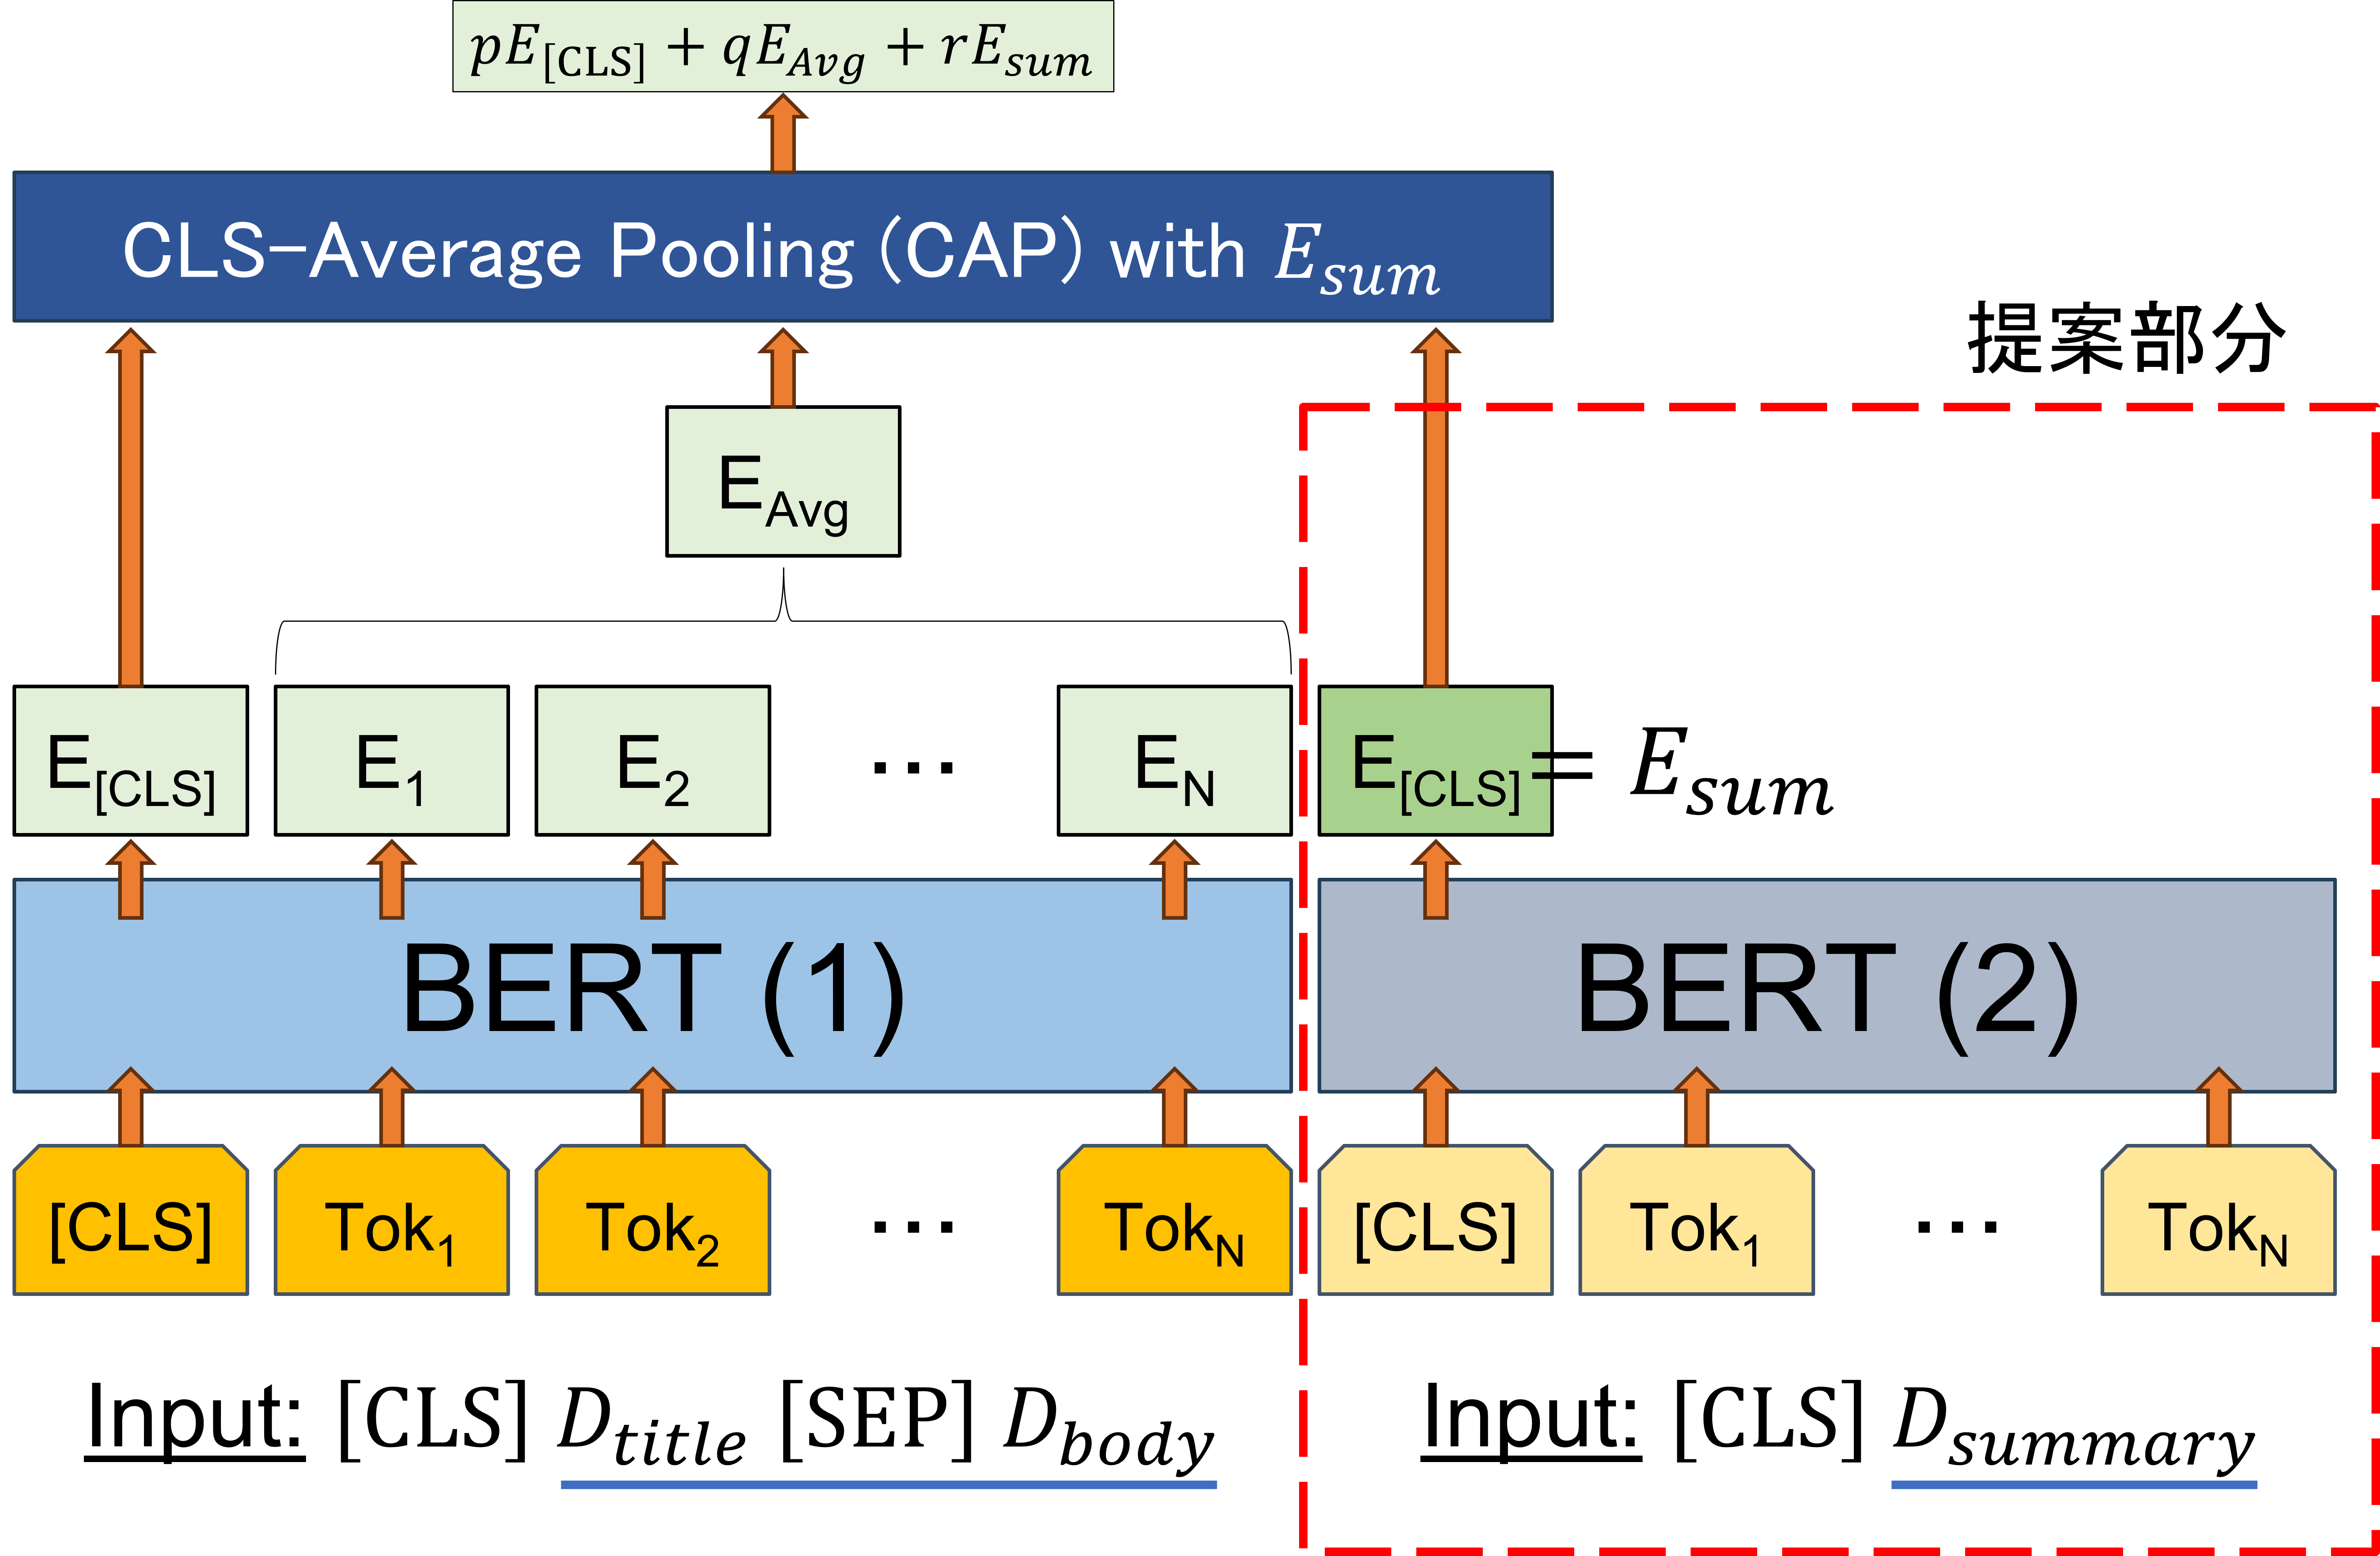
\includegraphics[width=1.0\linewidth]{tex_teian.png}
    \caption{提案手法モデルの概要} %タイトルをつける
    \label{fig:2_teian} %ラベルをつけ図の参照を可能にする
  \end{center}
\end{figure}

\begin{figure}[h]
  \begin{center}
    
\includegraphics[width=1.0\linewidth]{prompt.png}
    \caption{要約文の生成プロンプト} %タイトルをつける
    \label{fig:3_prompt} %ラベルをつけ図の参照を可能にする
  \end{center}
\end{figure}

そして, 図 \ref{fig:2_teian} のように 2 つの独立した事前学習済 BERT モデルを用いて, BERT (1) では原文データにおける [CLS] トークンの埋め込み表現 $E_{\rm{[CLS]}}$ および, [CLS] トークン以外の入力トークンすべてに対する平均プーリングによって得られた埋め込み表現 $E_{\rm{Avg}}$ を学習し, BERT (2) では要約文データにおける [CLS] トークンの埋め込み表現 $E_{\rm{sum}}$ を並行して学習して, 総和が 1 となる学習可能なパラメータ $p, q, r (\geq0)$ を用いて $E_{\rm{[CLS]}}$, $E_{\rm{Avg}}$, $E_{\rm{sum}}$ の重み付き和
\begin{equation}
  pE_{\rm{[CLS]}}+qE_{\rm{Avg}}+rE_{\rm{sum}}
\end{equation}
を入力データに対する分散表現とし, これを分類器への入力とする. また, 重みパラメータ $p, q, r$ の更新式は先行研究に倣い, 更新後の値を $p', q', r'$ とすると以下の式で表される.

\begin{equation}
  p' = \frac{p^{2}}{p^{2}+q^{2}+r^{2}}
\end{equation}
\begin{equation}
  q' = \frac{q^{2}}{p^{2}+q^{2}+r^{2}}
\end{equation}
\begin{equation}
  r' = \frac{r^{2}}{p^{2}+q^{2}+r^{2}}
\end{equation}


本研究では, 原文データにおいて記事タイトルと記事本文のペアを 1 文書として扱い, 各 BERT モデルへの入力形式は, 原文データを扱う BERT (1) では先行研究に倣って「 [CLS] $\rm{D_{\rm{title}}}$ [SEP] $\rm{D_{\rm{body}}}$」とし, 要約文データを扱う BERT (2) では「 [CLS] $\rm{D_{\rm{summary}}}$」の形式とした.

\section{数値実験}
本研究では, 提案手法の有効性を示すために, 先行研究と同様に livedoor ニュースコーパスの記事ラベルを推定するテキスト分類タスクを解き, 検証データにおける F1 値 が最も高いエポックにおけるモデルを用いてテストデータに対する精度を評価した. また, 精度比較のため従来手法として CAP 層のみを用いた場合と, 原文データを入力として使わずに, 要約文データにおける [CLS] トークンの埋め込み表現 $E_{\rm{sum}}$ のみを分類器への入力とした場合についても評価した. 表\ref{tab:params1} に実験パラメータを示す. 分類器は 1 層からなる全結合層とし, BERT (1) および BERT (2) についてはそれぞれの最終層のみをファインチューニングした.
\begin{table}[tp]
  \centering
  \caption{実験パラメータ}
 \scalebox{1.0}{
    \begin{tabular}{|c|c|}
    \hline
    パラメータ & 値 \\ \hline \hline
    最適化手法 & Adam \\ \hline
    学習率 & $3.0\times 10^{-5}$ \\ \hline
    損失関数 & Cross Entropy Loss \\ \hline
    エポック数 & 20 \\ \hline
    バッチサイズ & 16 \\ \hline
    最大トークン長 & 512 \\ \hline
    重み初期値 (提案手法) & $(p,q,r)=(\frac{1}{3},\frac{1}{3},\frac{1}{3})$ \\ \hline
    重み初期値 (従来手法) & $(p,q)=(0.5,0.5)$ \\ \hline
    \end{tabular}%
 }
  \label{tab:params1}%
\end{table}%

\begin{table}[t]
  \centering
  \caption{実験結果}
\begin{tabular}{l|cc}
\multicolumn{1}{c|}{\multirow{2}{*}{}} & \multicolumn{2}{c}{評価指標} \\ \cline{2-3}
\multicolumn{1}{c|}{} & \multicolumn{1}{c|}{Accuracy} & \begin{tabular}[c]{@{}c@{}}F1 値\\ (weighted)\end{tabular} \\ \hline
提案手法 & \multicolumn{1}{c|}{\underline{0.9687}} & \underline{0.9683} \\
従来手法 (CAP のみ) & \multicolumn{1}{c|}{0.9565} & 0.9560 \\
$E_{\rm{sum}}$ のみ & \multicolumn{1}{c|}{0.8369} & 0.8340 \\ \hline
ベースライン & \multicolumn{1}{c|}{0.1111} & -
\end{tabular}
\label{tab:result}
\end{table}

\begin{figure}[h]
  \begin{center}
    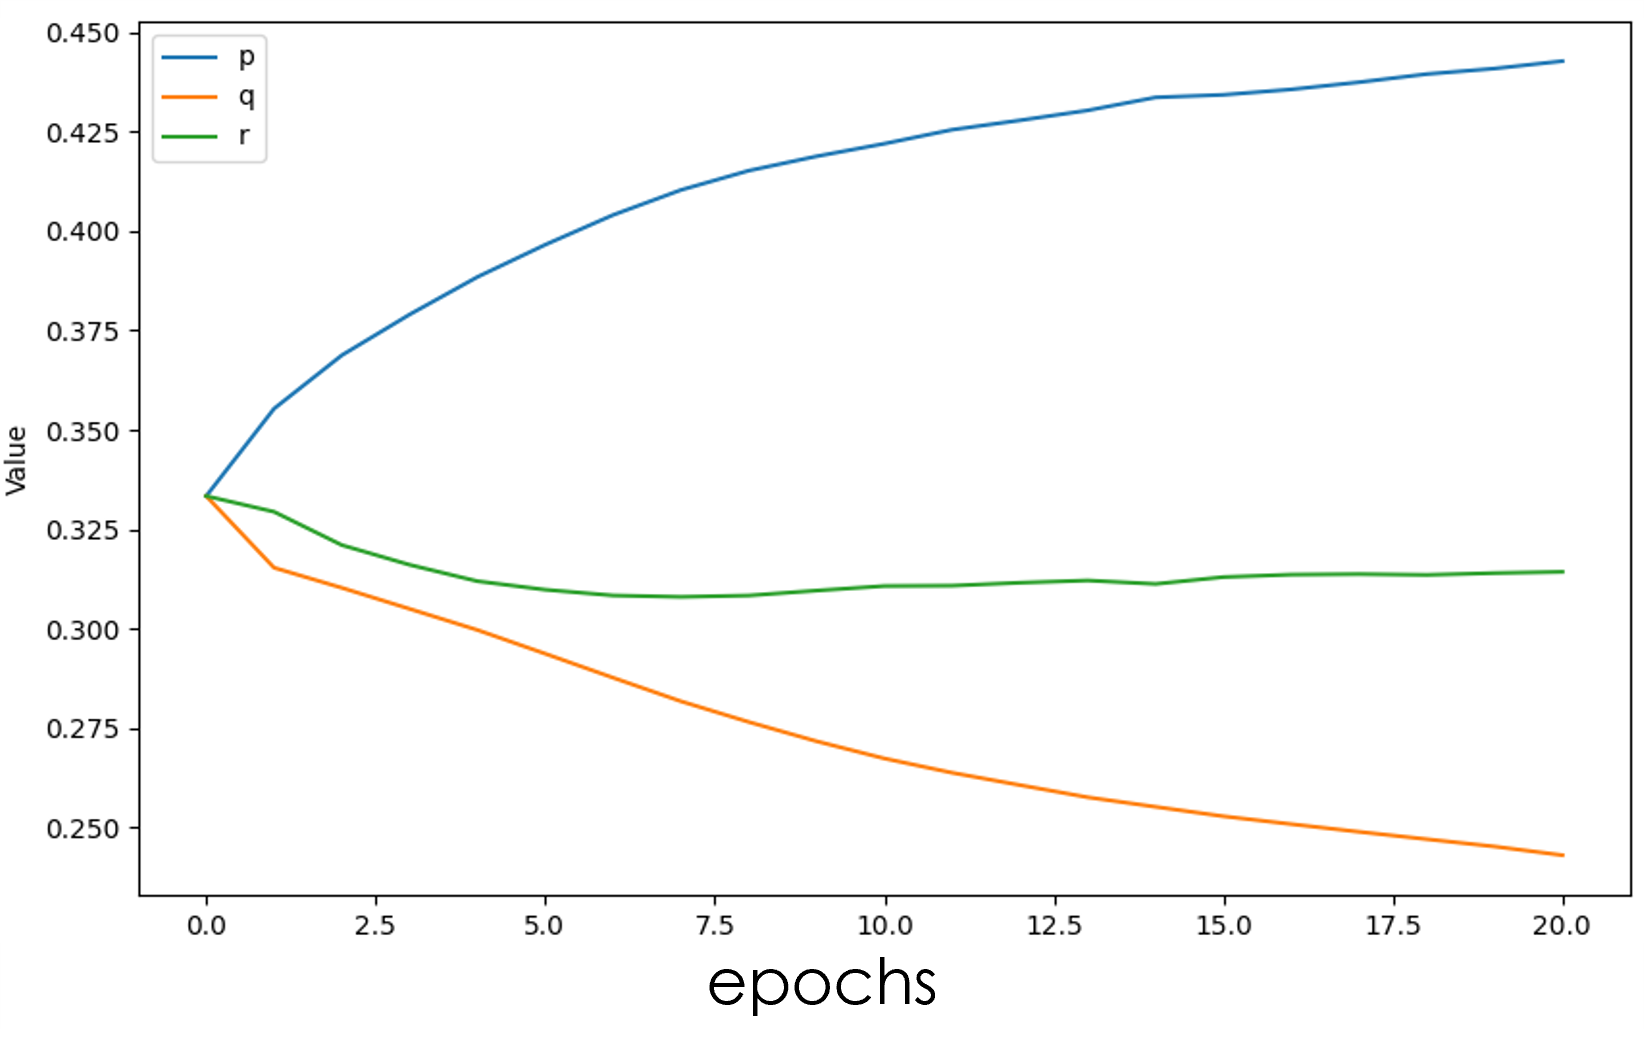
\includegraphics[width=1.0\linewidth]{pqr.png}
    \caption{パラメータ $(p, q, r)$ の学習推移} %タイトルをつける
    \label{fig:pqr} %ラベルをつけ図の参照を可能にする
  \end{center}
\end{figure}

\begin{figure}[h]
  \begin{center}
    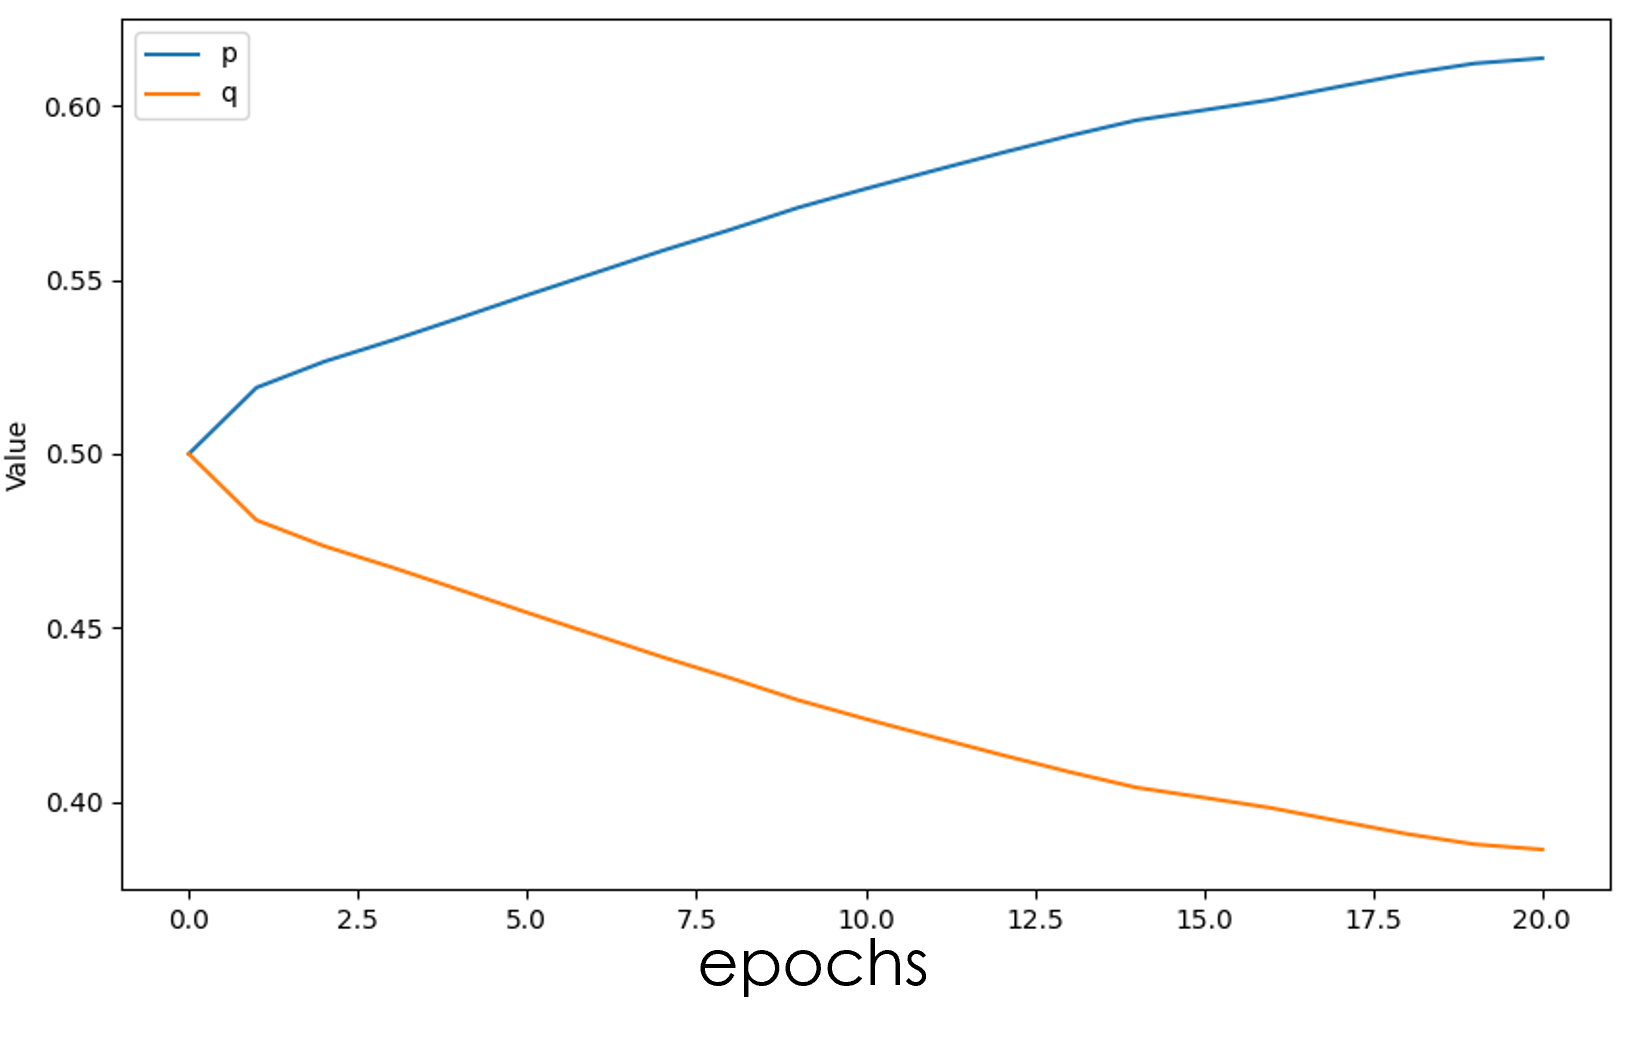
\includegraphics[width=1.0\linewidth]{pq.png}
    \caption{パラメータ $(p, q)$ の学習推移} %タイトルをつける
    \label{fig:pq} %ラベルをつけ図の参照を可能にする
  \end{center}
\end{figure}

\begin{figure}[th]
  \begin{center}
    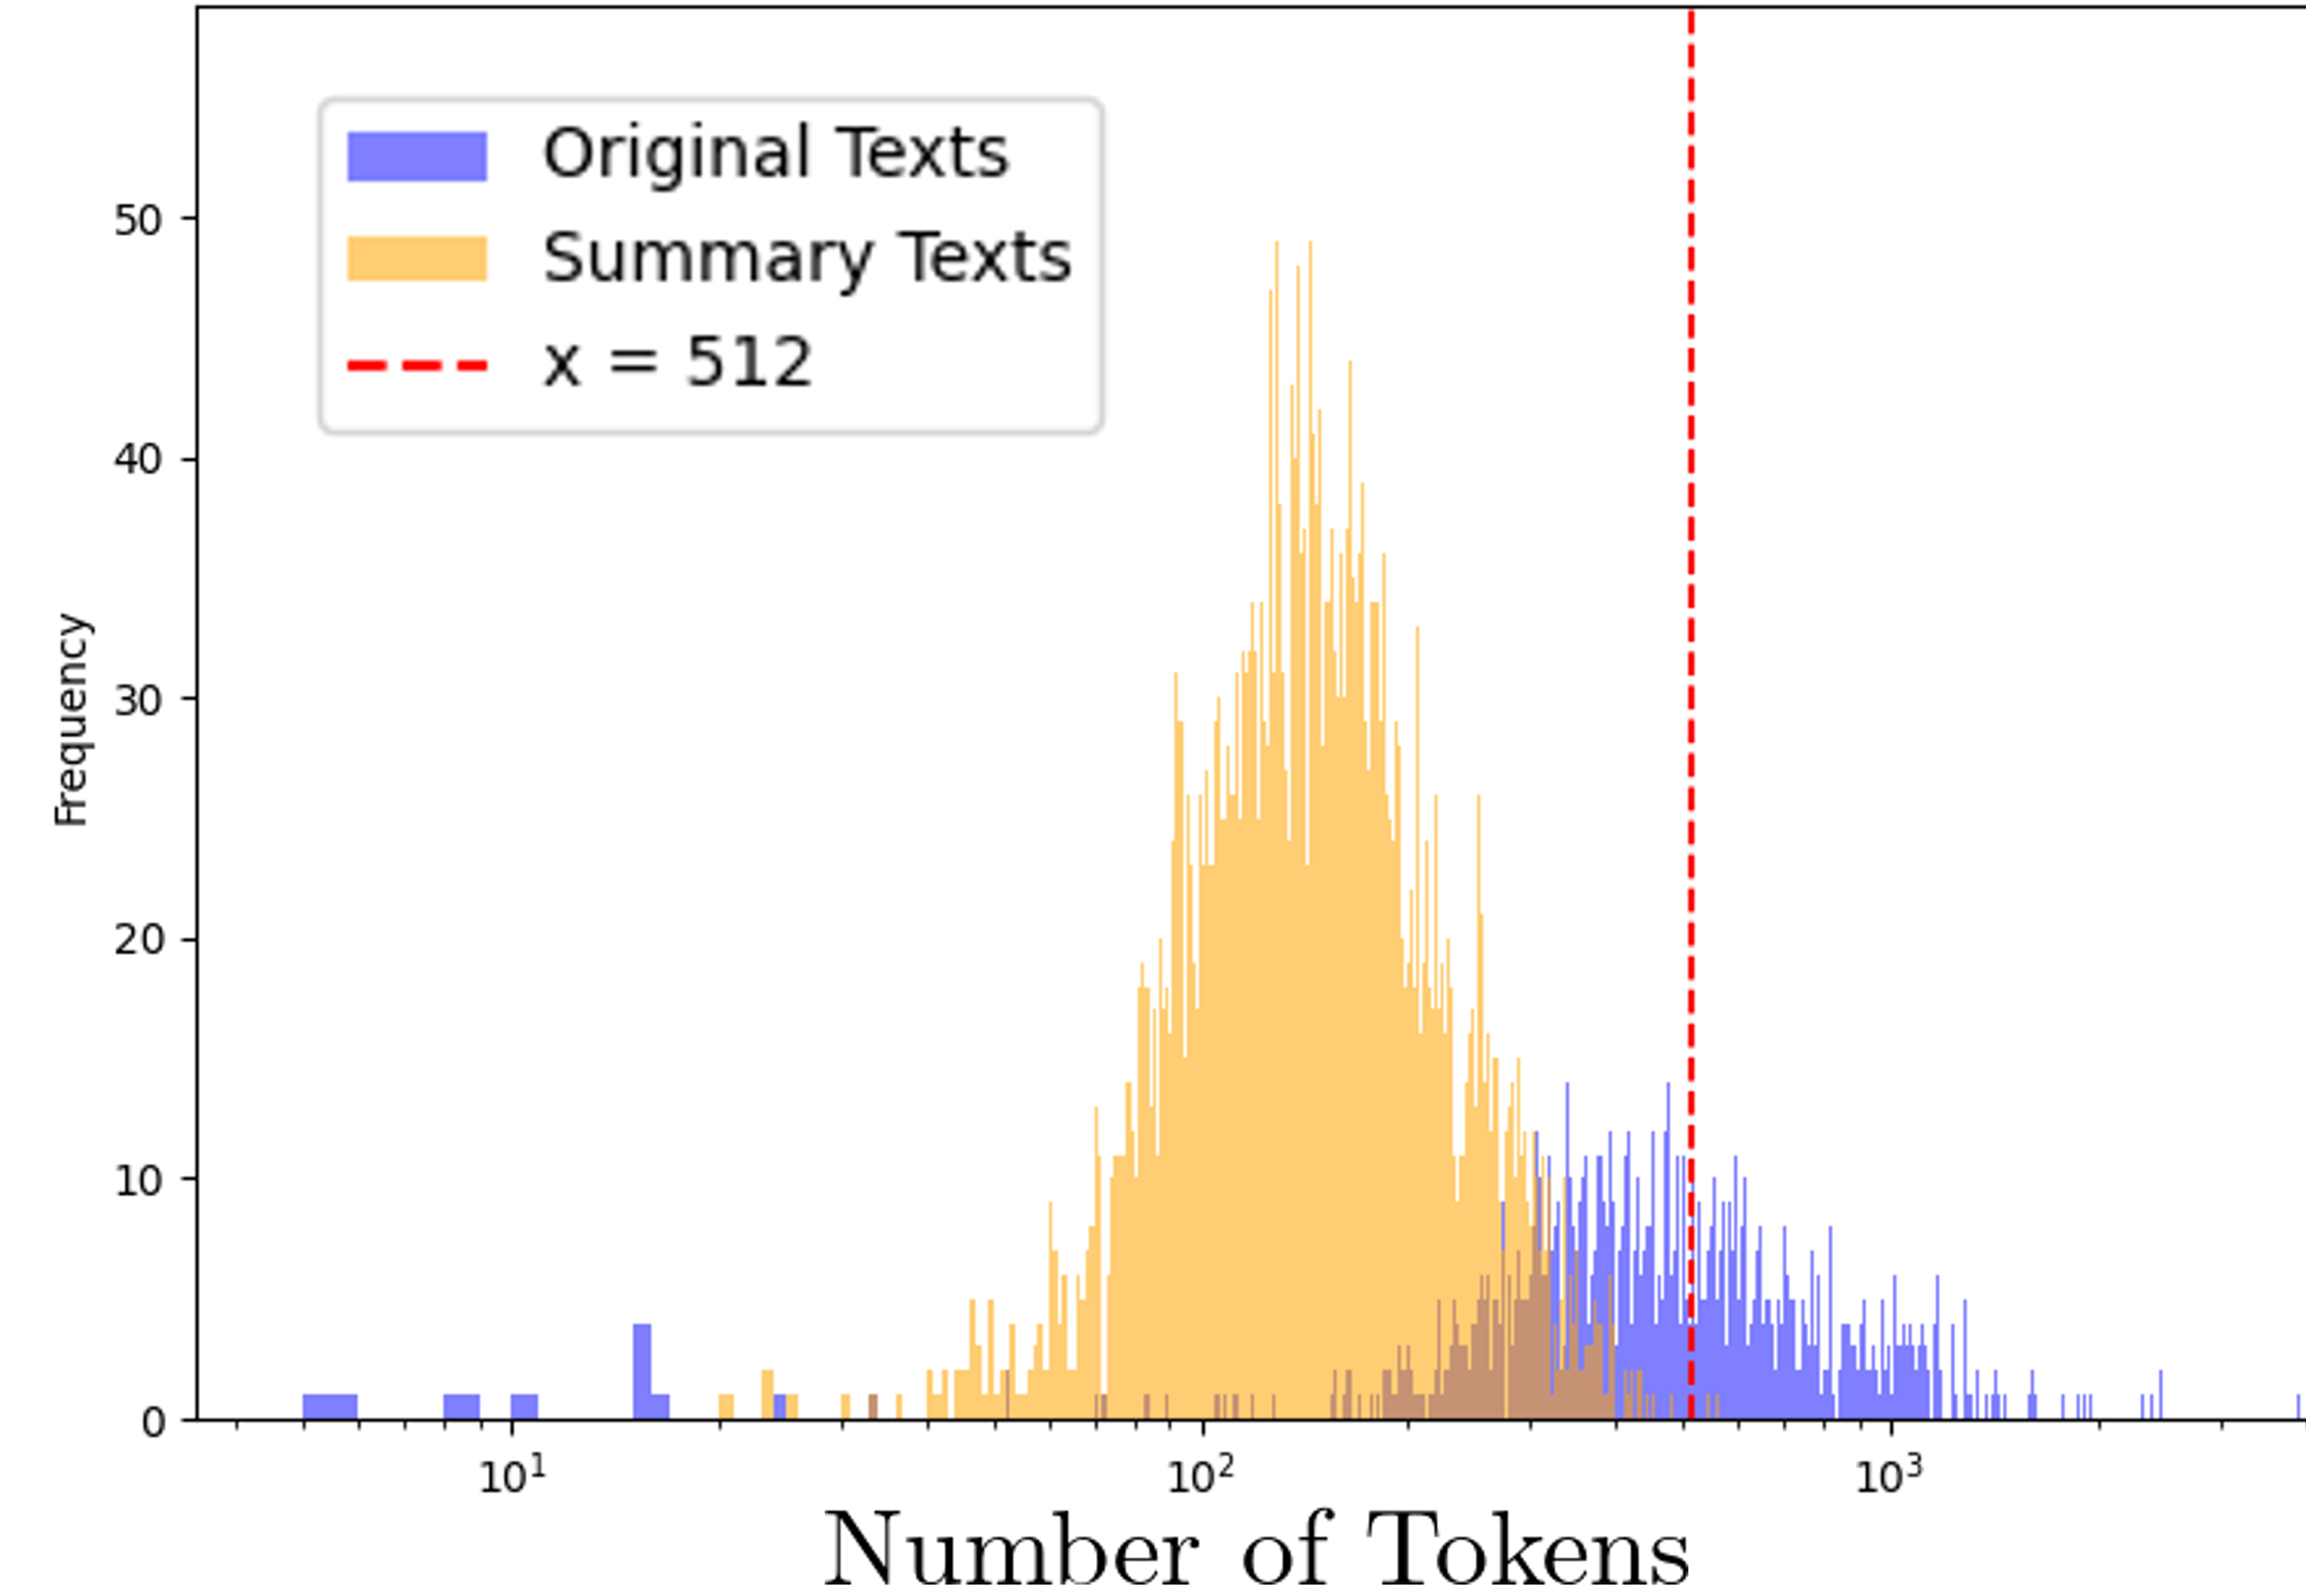
\includegraphics[width=1.0\linewidth]{token_num.png}
    \caption{訓練データにおけるトークン数分布} %タイトルをつける
    \label{fig:token_num} %ラベルをつけ図の参照を可能にする
  \end{center}
\end{figure}



表 \ref{tab:result} に実験結果を示す. ベースラインにはランダムでラベルを推定した場合を設定した. 表 \ref{tab:result} より, 提案手法における Accuracy は従来手法と比較して $0.0122$ ポイント向上しており, F1 値に関しても従来手法より $0.0123$ ポイント上回っている. $E_{\rm{sum}}$ のみを用いて推定した場合, 訓練データに対しては他の手法と同様に上手く学習が進んだが, 汎化性能が得られず高い評価指標を示さなかった.

次に, 図 \ref{fig:pqr} に提案手法におけるパラメータ $(p, q, r)$ の学習推移, 図 \ref{fig:pq} に従来手法におけるパラメータ $(p, q)$ の学習推移を示す. 縦軸はパラメータの値, 横軸はエポック数を示している. 最終エポックでの学習後におけるパラメータの値は, 提案手法では $(p, q, r) = (0.441, 0.245, 0.314)$ となり, 従来手法では $(p, q) = (0.613, 0.387)$ となった. 図 \ref{fig:pqr} および図 \ref{fig:pq} より, 原文データにおける [CLS] トークンの埋め込み表現 $E_{\rm{[CLS]}}$ の重み $p$ は単調増加し, [CLS] トークン以外の入力トークンすべてに対する平均プーリングによって得られた埋め込み表現 $E_{\rm{Avg}}$ の重み $q$ は単調減少していることが分かる. このことから, テキスト分類タスクにおいて, $E_{\rm{[CLS]}}$ は, $E_{\rm{Avg}}$ に比べて, 学習における重要度が高く, その重みが相対的に大きいことが分かる. そして, このタスクが $E_{\rm{[CLS]}}$ に強く依存しているのであれば, 提案手法において要約文データにおける [CLS] トークンの埋め込み表現 $E_{\rm{sum}}$ の重み $r$ に関しても単調に減少していくと考えられるが, 図 \ref{fig:pqr} より, $r$ の値は一定の値まで減少した後, わずかに増加する傾向が見られた. この結果より, $E_{\rm{sum}}$ が学習過程においてポジティブな寄与をしていることが分かった.

さらに, 図 \ref{fig:token_num} に訓練データにおけるトークン数の分布を示す. 縦軸は度数, 横軸は対数スケールでトークン数を示している. また, 紫色の分布が原文データ, 黄色の分布が要約文データのトークン数を表しており, 赤色の点線は本研究で使用している事前学習済 BERT モデルにおける最大入力トークン長である $512$ を示している. また, 表 \ref{tab:token_num_table} は図 \ref{fig:token_num} をもとに $512$ トークンを閾値としてデータ数を算出したものである. 表 \ref{tab:token_num_table} より, 原文データにおいて $512$ トークンを超えるデータは $3747$ 件あり, これは全体の約 $63\%$ を占めているのに対して, 要約文において $512$ トークンを超えるデータは $11$ 件しかなく, これは全体の約 $0.18\%$ と大幅に減少していることが分かった. このことから, 要約文データにおける [CLS] トークンの埋め込み表現 $E_{\rm{sum}}$ を学習に組み込むことで, 従来手法では学習時に欠損してしまっていた原文データの重要な文脈情報を補完したか, 原文データ内に含まれるキーワードが強調されたことによって分類精度の向上に貢献したと考えられる.

以上の結果より, 提案手法の有効性を確認することができた.

\begin{table}[!t]
\centering
\caption{トークン数が閾値より大きいかで分割した訓練データ数}
\begin{tabular}{l|cc}
\multicolumn{1}{c|}{\multirow{2}{*}{}} & \multicolumn{2}{c}{トークン数} \\ \cline{2-3}
\multicolumn{1}{c|}{} & \multicolumn{1}{c|}{$< 512$} & $\geq 512$ \\ \hline
原文データ & \multicolumn{1}{c|}{2148} & 3747 \\
要約文データ & \multicolumn{1}{c|}{5884} & 11
\end{tabular}
\label{tab:token_num_table}
\end{table}

\newpage
\section{まとめと今後の課題}
本研究では, 大和による [CLS] トークンの埋め込み表現を用いたプーリング手法と, 平均プーリング手法を組み合わせた CLS-Average Pooling (CAP 層) を基に, LLM を用いて生成した要約文の分散表現を組み込んだ新たなプーリング手法を提案し, テキスト分類タスクにおいて分類精度を検証した. その結果, Accuracy, F1 値ともに提案手法が高い評価指標を示し, その有効性を確認することができた.

今後の課題としては, 以下のものが挙げられる.
\begin{itemize}
  \item 要約文に対する妥当性の検討, および生成手法の改善\par
  \indent 本研究では PLaMo API のみを用いて原文データから要約文を生成したが, その妥当性については考慮していない. また, プロンプト内で回答の出力形式を自由にしていたため, 要約文データの一貫性を担保できていない. よって, 異なる LLM の活用や, 回答の出力形式をルールベースで厳格化することでより高品質な要約文が得られると考えられる.
  \item 他のタスクやデータセットにおける提案手法の有効性の検証\par
  \indent 本研究では livedoor ニュースコーパスデータセットを用いたテキスト分類において, 提案手法の有効性を示した.一方で他のタスクやデータセットにおける提案手法の有効性については不明瞭であるため, より複雑なデータセットや実験設定での検証が必要である.
\end{itemize}

\bibliography{bibliography}
\bibliographystyle{junsrt}

\end{document}
%%
